% =============================================================================
% cap5_resultados.tex
% Capítulo 5: Evaluación Experimental y Backtesting
% Para incluir en tfm.tex: % =============================================================================
% cap5_resultados.tex
% Capítulo 5: Evaluación Experimental y Backtesting
% Para incluir en tfm.tex: % =============================================================================
% cap5_resultados.tex
% Capítulo 5: Evaluación Experimental y Backtesting
% Para incluir en tfm.tex: % =============================================================================
% cap5_resultados.tex
% Capítulo 5: Evaluación Experimental y Backtesting
% Para incluir en tfm.tex: \input{cap5_resultados}
% =============================================================================

\section{Evaluación Experimental y Backtesting}

\subsection{Protocolo de Evaluación}

La validación del sistema se ha diseñado con el objetivo de aproximar, en la medida de lo posible, un entorno real de inversión. Para ello, se establecen una serie de criterios metodológicos orientados a evitar sesgos y a garantizar que la comparación entre estrategias sea homogénea.

\subsubsection{Causalidad temporal ($T/T+1$).}

Las decisiones de inversión se generan únicamente con la información disponible al cierre del último día hábil del período de rebalanceo $T$. La entrada efectiva en cartera se realiza al cierre del primer día hábil posterior ($T+1$). De esta forma, se evita incorporar información futura en el proceso de decisión.

Los retornos de cada cartera se calculan desde el cierre de $T+1$ hasta el cierre del siguiente período de rebalanceo. Además, todas las transformaciones estadísticas utilizadas por el modelo (como los \textit{Rolling Z-Scores}) se estiman exclusivamente con datos históricos disponibles en cada fecha.

\subsubsection{Benchmark de referencia.}

Como índice de comparación se utiliza el ETF \textit{SPDR S\&P 500 ETF Trust} (SPY), ampliamente empleado como referencia representativa de la renta variable estadounidense. Su curva de capital se normaliza a base 1,0 en la misma fecha inicial que la estrategia, permitiendo una comparación directa y visual del comportamiento acumulado.

\subsubsection{Construcción de cartera mediante ranking.}

Una vez identificado el régimen de mercado y seleccionados los activos candidatos, la ponderación interna de la cartera no se realiza a partes iguales, sino mediante un sistema decreciente por ranking. Los activos con mejor puntuación de \textit{momentum} reciben un mayor peso relativo.

En cada fecha de rebalanceo, la estrategia selecciona los diez activos mejor posicionados según el criterio de ranking definido por el modelo, dando lugar a una cartera \textit{Top-10}. Este enfoque busca combinar concentración en las señales más sólidas con un nivel razonable de diversificación, evitando depender excesivamente de un número muy reducido de posiciones.

\begin{equation}
w_i = \frac{N+1-i}{\displaystyle\sum_{j=1}^{N} j}, \qquad i=1,2,\dots,N
\end{equation}

donde $i=1$ representa el activo mejor clasificado y $N$ el número total de posiciones. En este caso, al emplearse una cartera \textit{Top-10}, se tiene $N=10$. Este esquema permite concentrar algo más de exposición en las señales más fuertes, manteniendo al mismo tiempo diversificación.

\subsection{Desempeño por Régimen}

La Figura \ref{fig:capital_clusters} muestra la evolución acumulada de capital para cada uno de los cinco regímenes detectados por K-Means, utilizando rebalanceo mensual, selección Top-5 y ponderación por ranking.

\begin{figure}[H]
    \centering
    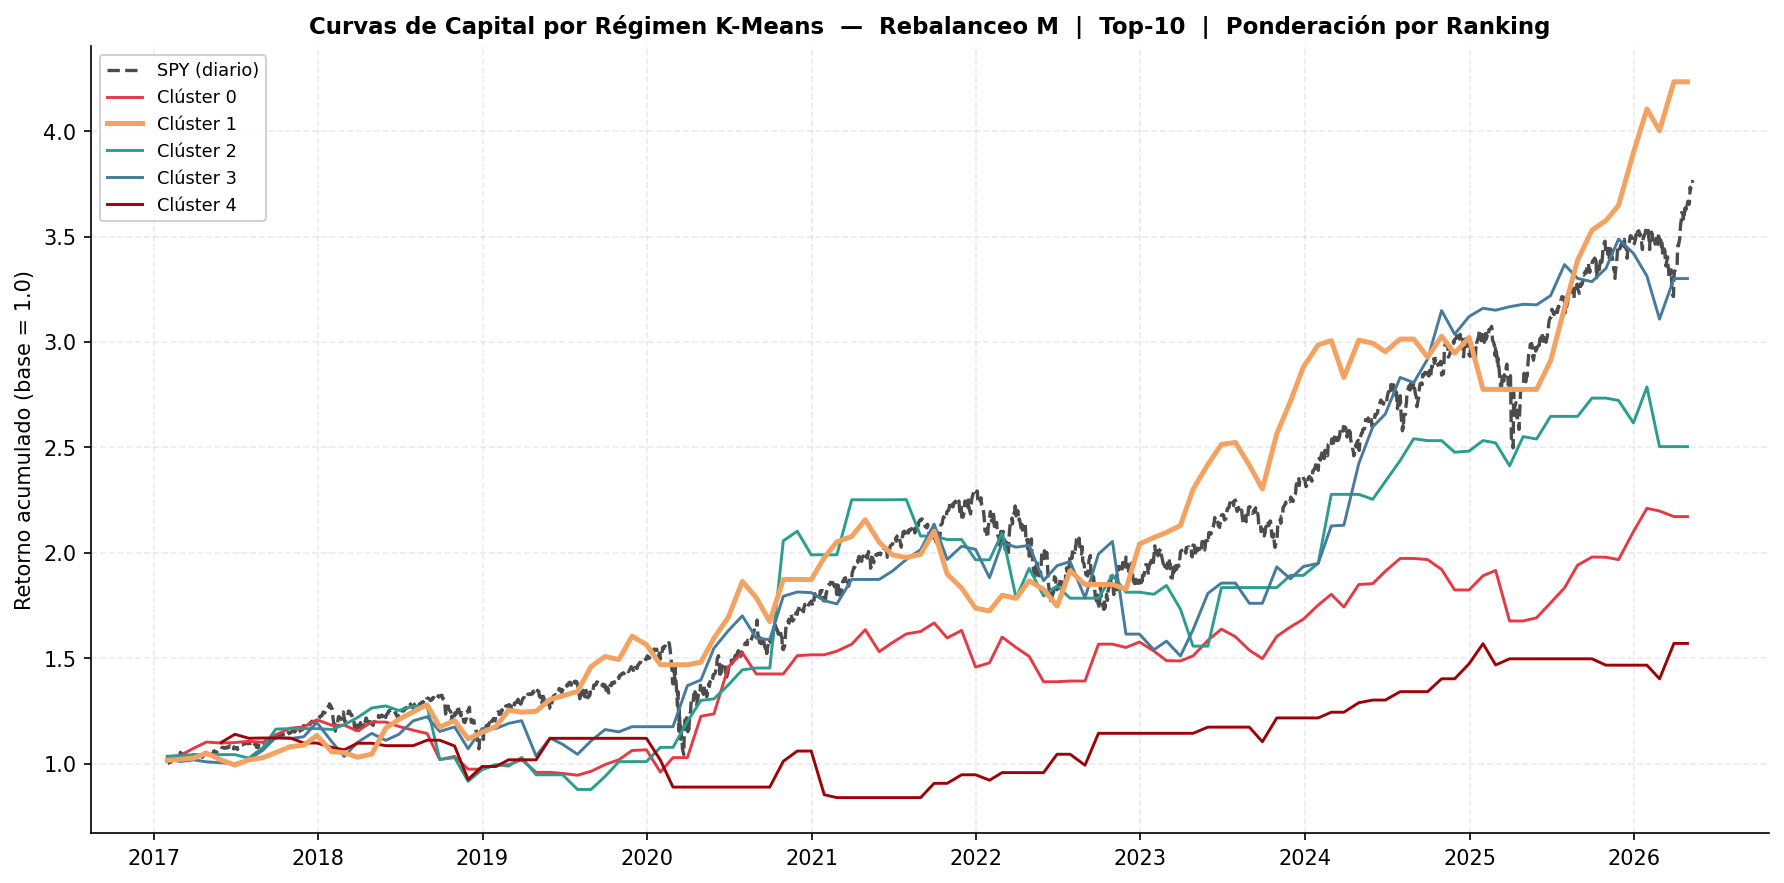
\includegraphics[width=0.95\textwidth]{media/equity_simple.png}
    \caption{Curvas de capital por régimen K-Means frente al benchmark SPY.}
    \label{fig:capital_clusters}
\end{figure}

De forma visual ya se aprecia que no todos los entornos de mercado ofrecen las mismas condiciones para una estrategia basada en \textit{momentum}. Algunos clústeres concentran fases especialmente favorables, mientras que otros presentan resultados más discretos o mayor inestabilidad.

\begin{table}[H]
\centering
\caption{Métricas principales por régimen de mercado. Rebalanceo mensual, Top-10 y ponderación por ranking.}
\label{tab:metricas_clusters}
\resizebox{\textwidth}{!}{%  <--- ESTA LÍNEA ES LA MAGIA
\begin{tabular}{lccccc}
\toprule
\textbf{Clúster} & \textbf{CAGR (\%)} & \textbf{Sharpe} & \textbf{MaxDD (\%)} & \textbf{Períodos Activos} & \textbf{SPY CAGR (\%)} \\
\midrule
0 --- Bajista moderado      & 8,66  & 0,531 & -21,80 & 97  & 11,79 \\
1 --- Bear market rally     & 16,72 & 1,002 & -20,06 & 101 & 11,79 \\
2 --- Alcista estable       & 10,33 & 0,462 & -31,13 & 74  & 11,79 \\
3 --- Pullback alcista      & 13,65 & 0,664 & -29,29 & 102 & 11,79 \\
4 --- Estrés/Capitulación   & 5,14  & 0,312 & -26,39 & 44  & 11,79 \\
\bottomrule
\end{tabular}
} % <--- NO TE OLVIDES DE CERRAR LA LLAVE AQUÍ
\end{table}

Los resultados, calculados mediante una diversificación \textit{Top-10}, muestran una diferenciación cuantitativa clara entre regímenes:

\begin{itemize}
    \item \textbf{Clúster 1 (Bear market rally):} Presenta el mejor comportamiento agregado de forma destacada, con un CAGR del 16,72\% y un ratio Sharpe de 1,002, batiendo ampliamente al \textit{benchmark}. El análisis de sus activos constituyentes más frecuentes (ej. Banco Santander, Ferrovial y activos defensivos como el oro a través de GLD) sugiere que, tras fases de sobreventa, las rotaciones agresivas hacia activos descorrelacionados o cíclicos ofrecen un \textit{alpha} significativo.
    
    \item \textbf{Clúster 3 (Pullback alcista):} Se consolida como un régimen altamente favorable, superando también al SPY con un CAGR del 13,65\% y un Sharpe robusto (0,664) respaldado por 102 períodos activos. Este dato confirma que comprar líderes de \textit{momentum} durante pequeñas correcciones dentro de tendencias estructurales positivas es una de las estrategias estadísticamente más fiables.
    
    \item \textbf{Clúster 2 (Alcista estable):} Muestra una rentabilidad positiva (10,33\%), pero ligeramente inferior al SPY. En mercados extremadamente complacientes y ordenados, el modelo \textit{Top-10} sufre porque la dispersión entre activos es menor; es decir, "todo sube", lo que diluye la ventaja comparativa del factor \textit{momentum}.
    
    \item \textbf{Clústeres 0 y 4 (Regímenes de debilidad y estrés):} Presentan los peores resultados relativos. Destaca especialmente el Clúster 4 (Capitulación), con apenas un 5,14\% de CAGR y un Sharpe deficiente de 0,312. Además, al observar los activos seleccionados durante este clúster (los propios índices SPY y QQQ), se infiere que el algoritmo colapsa y no encuentra acciones individuales que destaquen, refugiándose en el mercado general en medio del pánico.
\end{itemize}

En conjunto, los datos respaldan la idea central del trabajo: la rentabilidad ajustada al riesgo del factor \textit{momentum} no es constante, sino fuertemente asimétrica y dependiente del régimen de mercado detectado mediante K-Means.


% \parencite{Daniel2016}
% \parencite{Asness2013}

\subsection{Interpretación Económica de los Regímenes}

Más allá de la rentabilidad, los clústeres detectados presentan una lectura económica coherente:

\begin{itemize}
    \item \textbf{Bajista moderado:} fases de deterioro, sin capitulación extrema.
    
    \item \textbf{Bear market rally:} rebotes intensos tras caídas previas, normalmente acompañados de alta dispersión entre activos.
    
    \item \textbf{Alcista estable:} tendencia positiva sostenida, con volatilidad relativamente contenida.
    
    \item \textbf{Pullback alcista:} correcciones temporales dentro de un mercado estructuralmente favorable.
    
    \item \textbf{Estrés/Capitulación:} episodios de miedo generalizado, ventas forzadas o shocks externos.
\end{itemize}

Esta clasificación refuerza que el algoritmo no solo segmenta datos estadísticamente, sino que identifica contextos reconocibles desde el punto de vista financiero.

\subsection{Implicaciones para la Gestión de Cartera}

Una de las conclusiones más relevantes es que no todos los regímenes justifican el mismo nivel de exposición al riesgo. Si determinados clústeres concentran mejores métricas históricas, una aplicación práctica del modelo consistiría en modular el tamaño de la posición según el entorno detectado.

Por ejemplo:

\begin{itemize}
    \item Mayor exposición en clústeres 1 y 3.
    \item Exposición neutral o reducida en clúster 2.
    \item Perfil defensivo o incluso ausencia de señal en clústeres 0 y 4.
\end{itemize}

Este enfoque convertiría al sistema en una herramienta no solo de selección de activos, sino también de asignación.

%\subsection{Conclusión del Capítulo}

%Los resultados obtenidos muestran que la combinación de filtrado topológico (DBSCAN), segmentación por regímenes (K-Means) y selección por \textit{momentum} genera comportamientos diferenciados y económicamente interpretables.

%La evidencia empírica sugiere que adaptar la estrategia al contexto de mercado mejora la consistencia de los resultados frente a una aplicación indiscriminada del mismo modelo en cualquier entorno. En consecuencia, la detección previa del régimen se confirma como una capa de valor relevante dentro de la arquitectura propuesta.
% =============================================================================

\section{Evaluación Experimental y Backtesting}

\subsection{Protocolo de Evaluación}

La validación del sistema se ha diseñado con el objetivo de aproximar, en la medida de lo posible, un entorno real de inversión. Para ello, se establecen una serie de criterios metodológicos orientados a evitar sesgos y a garantizar que la comparación entre estrategias sea homogénea.

\subsubsection{Causalidad temporal ($T/T+1$).}

Las decisiones de inversión se generan únicamente con la información disponible al cierre del último día hábil del período de rebalanceo $T$. La entrada efectiva en cartera se realiza al cierre del primer día hábil posterior ($T+1$). De esta forma, se evita incorporar información futura en el proceso de decisión.

Los retornos de cada cartera se calculan desde el cierre de $T+1$ hasta el cierre del siguiente período de rebalanceo. Además, todas las transformaciones estadísticas utilizadas por el modelo (como los \textit{Rolling Z-Scores}) se estiman exclusivamente con datos históricos disponibles en cada fecha.

\subsubsection{Benchmark de referencia.}

Como índice de comparación se utiliza el ETF \textit{SPDR S\&P 500 ETF Trust} (SPY), ampliamente empleado como referencia representativa de la renta variable estadounidense. Su curva de capital se normaliza a base 1,0 en la misma fecha inicial que la estrategia, permitiendo una comparación directa y visual del comportamiento acumulado.

\subsubsection{Construcción de cartera mediante ranking.}

Una vez identificado el régimen de mercado y seleccionados los activos candidatos, la ponderación interna de la cartera no se realiza a partes iguales, sino mediante un sistema decreciente por ranking. Los activos con mejor puntuación de \textit{momentum} reciben un mayor peso relativo.

En cada fecha de rebalanceo, la estrategia selecciona los diez activos mejor posicionados según el criterio de ranking definido por el modelo, dando lugar a una cartera \textit{Top-10}. Este enfoque busca combinar concentración en las señales más sólidas con un nivel razonable de diversificación, evitando depender excesivamente de un número muy reducido de posiciones.

\begin{equation}
w_i = \frac{N+1-i}{\displaystyle\sum_{j=1}^{N} j}, \qquad i=1,2,\dots,N
\end{equation}

donde $i=1$ representa el activo mejor clasificado y $N$ el número total de posiciones. En este caso, al emplearse una cartera \textit{Top-10}, se tiene $N=10$. Este esquema permite concentrar algo más de exposición en las señales más fuertes, manteniendo al mismo tiempo diversificación.

\subsection{Desempeño por Régimen}

La Figura \ref{fig:capital_clusters} muestra la evolución acumulada de capital para cada uno de los cinco regímenes detectados por K-Means, utilizando rebalanceo mensual, selección Top-5 y ponderación por ranking.

\begin{figure}[H]
    \centering
    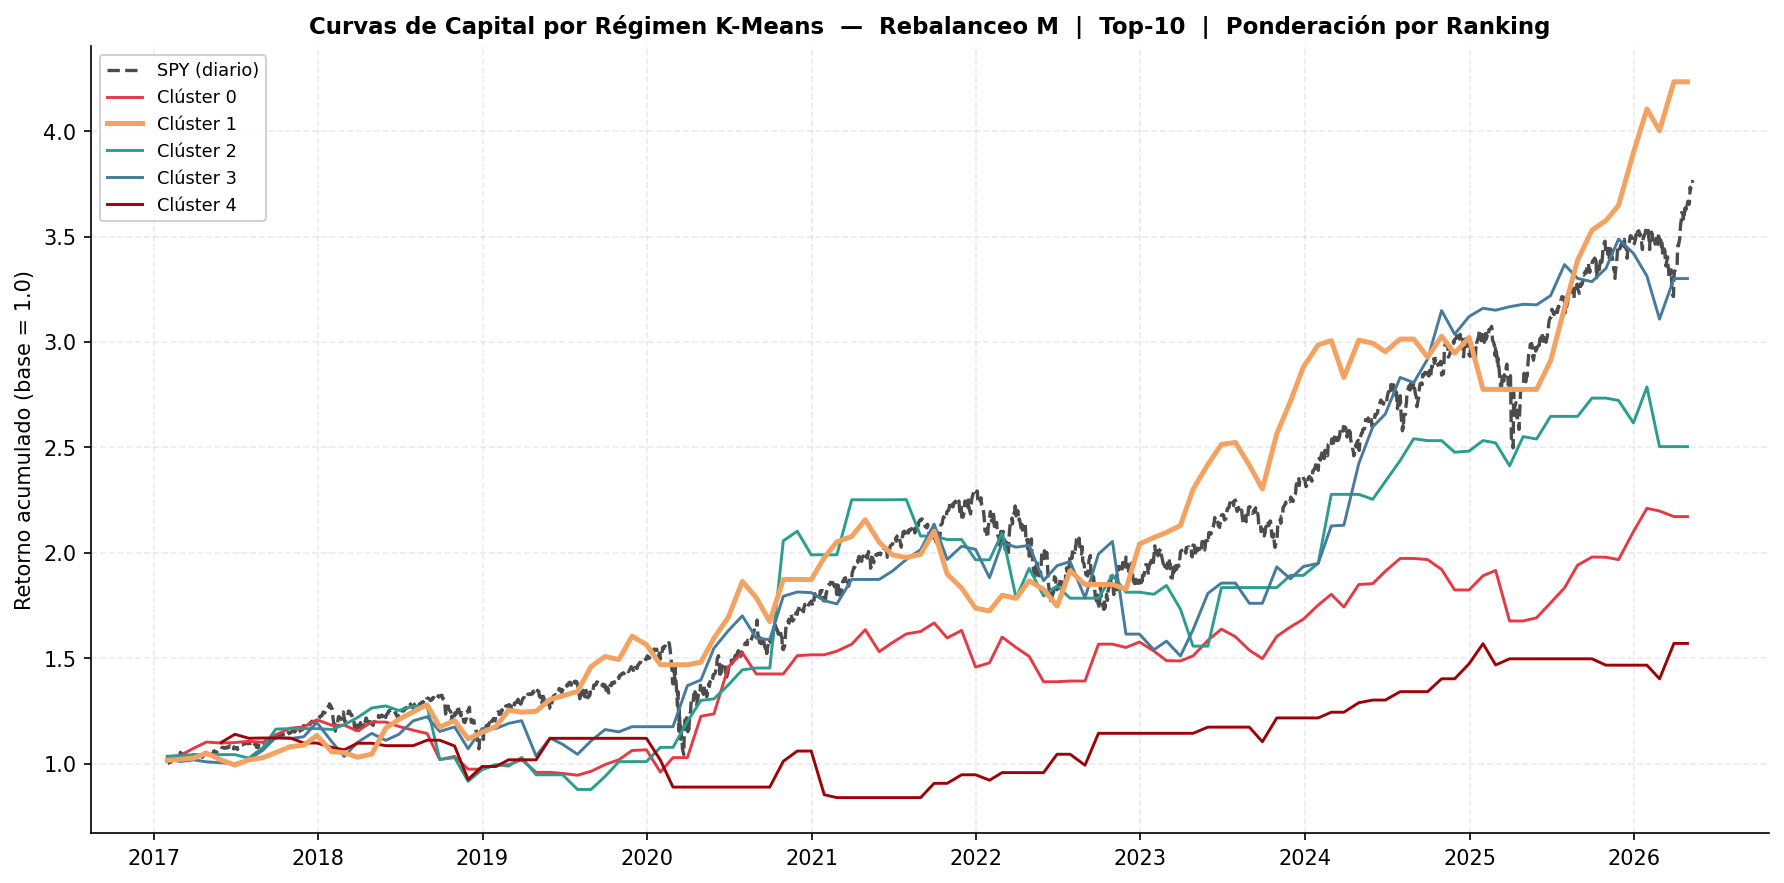
\includegraphics[width=0.95\textwidth]{media/equity_simple.png}
    \caption{Curvas de capital por régimen K-Means frente al benchmark SPY.}
    \label{fig:capital_clusters}
\end{figure}

De forma visual ya se aprecia que no todos los entornos de mercado ofrecen las mismas condiciones para una estrategia basada en \textit{momentum}. Algunos clústeres concentran fases especialmente favorables, mientras que otros presentan resultados más discretos o mayor inestabilidad.

\begin{table}[H]
\centering
\caption{Métricas principales por régimen de mercado. Rebalanceo mensual, Top-10 y ponderación por ranking.}
\label{tab:metricas_clusters}
\resizebox{\textwidth}{!}{%  <--- ESTA LÍNEA ES LA MAGIA
\begin{tabular}{lccccc}
\toprule
\textbf{Clúster} & \textbf{CAGR (\%)} & \textbf{Sharpe} & \textbf{MaxDD (\%)} & \textbf{Períodos Activos} & \textbf{SPY CAGR (\%)} \\
\midrule
0 --- Bajista moderado      & 8,66  & 0,531 & -21,80 & 97  & 11,79 \\
1 --- Bear market rally     & 16,72 & 1,002 & -20,06 & 101 & 11,79 \\
2 --- Alcista estable       & 10,33 & 0,462 & -31,13 & 74  & 11,79 \\
3 --- Pullback alcista      & 13,65 & 0,664 & -29,29 & 102 & 11,79 \\
4 --- Estrés/Capitulación   & 5,14  & 0,312 & -26,39 & 44  & 11,79 \\
\bottomrule
\end{tabular}
} % <--- NO TE OLVIDES DE CERRAR LA LLAVE AQUÍ
\end{table}

Los resultados, calculados mediante una diversificación \textit{Top-10}, muestran una diferenciación cuantitativa clara entre regímenes:

\begin{itemize}
    \item \textbf{Clúster 1 (Bear market rally):} Presenta el mejor comportamiento agregado de forma destacada, con un CAGR del 16,72\% y un ratio Sharpe de 1,002, batiendo ampliamente al \textit{benchmark}. El análisis de sus activos constituyentes más frecuentes (ej. Banco Santander, Ferrovial y activos defensivos como el oro a través de GLD) sugiere que, tras fases de sobreventa, las rotaciones agresivas hacia activos descorrelacionados o cíclicos ofrecen un \textit{alpha} significativo.
    
    \item \textbf{Clúster 3 (Pullback alcista):} Se consolida como un régimen altamente favorable, superando también al SPY con un CAGR del 13,65\% y un Sharpe robusto (0,664) respaldado por 102 períodos activos. Este dato confirma que comprar líderes de \textit{momentum} durante pequeñas correcciones dentro de tendencias estructurales positivas es una de las estrategias estadísticamente más fiables.
    
    \item \textbf{Clúster 2 (Alcista estable):} Muestra una rentabilidad positiva (10,33\%), pero ligeramente inferior al SPY. En mercados extremadamente complacientes y ordenados, el modelo \textit{Top-10} sufre porque la dispersión entre activos es menor; es decir, "todo sube", lo que diluye la ventaja comparativa del factor \textit{momentum}.
    
    \item \textbf{Clústeres 0 y 4 (Regímenes de debilidad y estrés):} Presentan los peores resultados relativos. Destaca especialmente el Clúster 4 (Capitulación), con apenas un 5,14\% de CAGR y un Sharpe deficiente de 0,312. Además, al observar los activos seleccionados durante este clúster (los propios índices SPY y QQQ), se infiere que el algoritmo colapsa y no encuentra acciones individuales que destaquen, refugiándose en el mercado general en medio del pánico.
\end{itemize}

En conjunto, los datos respaldan la idea central del trabajo: la rentabilidad ajustada al riesgo del factor \textit{momentum} no es constante, sino fuertemente asimétrica y dependiente del régimen de mercado detectado mediante K-Means.


% \parencite{Daniel2016}
% \parencite{Asness2013}

\subsection{Interpretación Económica de los Regímenes}

Más allá de la rentabilidad, los clústeres detectados presentan una lectura económica coherente:

\begin{itemize}
    \item \textbf{Bajista moderado:} fases de deterioro, sin capitulación extrema.
    
    \item \textbf{Bear market rally:} rebotes intensos tras caídas previas, normalmente acompañados de alta dispersión entre activos.
    
    \item \textbf{Alcista estable:} tendencia positiva sostenida, con volatilidad relativamente contenida.
    
    \item \textbf{Pullback alcista:} correcciones temporales dentro de un mercado estructuralmente favorable.
    
    \item \textbf{Estrés/Capitulación:} episodios de miedo generalizado, ventas forzadas o shocks externos.
\end{itemize}

Esta clasificación refuerza que el algoritmo no solo segmenta datos estadísticamente, sino que identifica contextos reconocibles desde el punto de vista financiero.

\subsection{Implicaciones para la Gestión de Cartera}

Una de las conclusiones más relevantes es que no todos los regímenes justifican el mismo nivel de exposición al riesgo. Si determinados clústeres concentran mejores métricas históricas, una aplicación práctica del modelo consistiría en modular el tamaño de la posición según el entorno detectado.

Por ejemplo:

\begin{itemize}
    \item Mayor exposición en clústeres 1 y 3.
    \item Exposición neutral o reducida en clúster 2.
    \item Perfil defensivo o incluso ausencia de señal en clústeres 0 y 4.
\end{itemize}

Este enfoque convertiría al sistema en una herramienta no solo de selección de activos, sino también de asignación.

%\subsection{Conclusión del Capítulo}

%Los resultados obtenidos muestran que la combinación de filtrado topológico (DBSCAN), segmentación por regímenes (K-Means) y selección por \textit{momentum} genera comportamientos diferenciados y económicamente interpretables.

%La evidencia empírica sugiere que adaptar la estrategia al contexto de mercado mejora la consistencia de los resultados frente a una aplicación indiscriminada del mismo modelo en cualquier entorno. En consecuencia, la detección previa del régimen se confirma como una capa de valor relevante dentro de la arquitectura propuesta.
% =============================================================================

\section{Evaluación Experimental y Backtesting}

\subsection{Protocolo de Evaluación}

La validación del sistema se ha diseñado con el objetivo de aproximar, en la medida de lo posible, un entorno real de inversión. Para ello, se establecen una serie de criterios metodológicos orientados a evitar sesgos y a garantizar que la comparación entre estrategias sea homogénea.

\subsubsection{Causalidad temporal ($T/T+1$).}

Las decisiones de inversión se generan únicamente con la información disponible al cierre del último día hábil del período de rebalanceo $T$. La entrada efectiva en cartera se realiza al cierre del primer día hábil posterior ($T+1$). De esta forma, se evita incorporar información futura en el proceso de decisión.

Los retornos de cada cartera se calculan desde el cierre de $T+1$ hasta el cierre del siguiente período de rebalanceo. Además, todas las transformaciones estadísticas utilizadas por el modelo (como los \textit{Rolling Z-Scores}) se estiman exclusivamente con datos históricos disponibles en cada fecha.

\subsubsection{Benchmark de referencia.}

Como índice de comparación se utiliza el ETF \textit{SPDR S\&P 500 ETF Trust} (SPY), ampliamente empleado como referencia representativa de la renta variable estadounidense. Su curva de capital se normaliza a base 1,0 en la misma fecha inicial que la estrategia, permitiendo una comparación directa y visual del comportamiento acumulado.

\subsubsection{Construcción de cartera mediante ranking.}

Una vez identificado el régimen de mercado y seleccionados los activos candidatos, la ponderación interna de la cartera no se realiza a partes iguales, sino mediante un sistema decreciente por ranking. Los activos con mejor puntuación de \textit{momentum} reciben un mayor peso relativo.

En cada fecha de rebalanceo, la estrategia selecciona los diez activos mejor posicionados según el criterio de ranking definido por el modelo, dando lugar a una cartera \textit{Top-10}. Este enfoque busca combinar concentración en las señales más sólidas con un nivel razonable de diversificación, evitando depender excesivamente de un número muy reducido de posiciones.

\begin{equation}
w_i = \frac{N+1-i}{\displaystyle\sum_{j=1}^{N} j}, \qquad i=1,2,\dots,N
\end{equation}

donde $i=1$ representa el activo mejor clasificado y $N$ el número total de posiciones. En este caso, al emplearse una cartera \textit{Top-10}, se tiene $N=10$. Este esquema permite concentrar algo más de exposición en las señales más fuertes, manteniendo al mismo tiempo diversificación.

\subsection{Desempeño por Régimen}

La Figura \ref{fig:capital_clusters} muestra la evolución acumulada de capital para cada uno de los cinco regímenes detectados por K-Means, utilizando rebalanceo mensual, selección Top-5 y ponderación por ranking.

\begin{figure}[H]
    \centering
    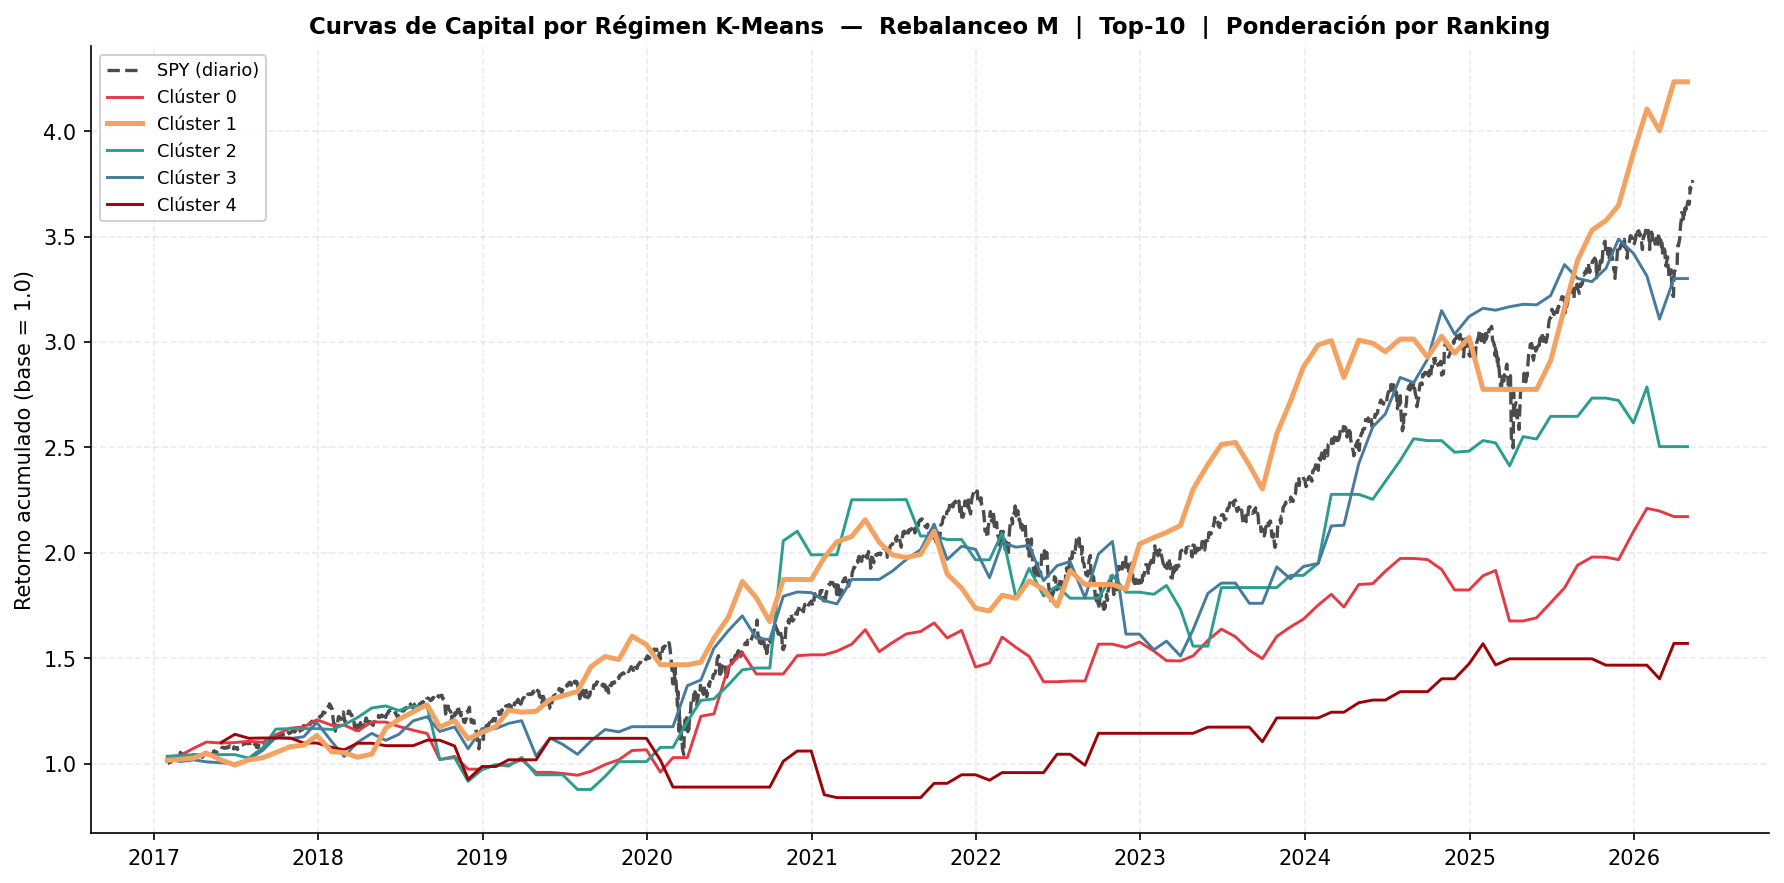
\includegraphics[width=0.95\textwidth]{media/equity_simple.png}
    \caption{Curvas de capital por régimen K-Means frente al benchmark SPY.}
    \label{fig:capital_clusters}
\end{figure}

De forma visual ya se aprecia que no todos los entornos de mercado ofrecen las mismas condiciones para una estrategia basada en \textit{momentum}. Algunos clústeres concentran fases especialmente favorables, mientras que otros presentan resultados más discretos o mayor inestabilidad.

\begin{table}[H]
\centering
\caption{Métricas principales por régimen de mercado. Rebalanceo mensual, Top-10 y ponderación por ranking.}
\label{tab:metricas_clusters}
\resizebox{\textwidth}{!}{%  <--- ESTA LÍNEA ES LA MAGIA
\begin{tabular}{lccccc}
\toprule
\textbf{Clúster} & \textbf{CAGR (\%)} & \textbf{Sharpe} & \textbf{MaxDD (\%)} & \textbf{Períodos Activos} & \textbf{SPY CAGR (\%)} \\
\midrule
0 --- Bajista moderado      & 8,66  & 0,531 & -21,80 & 97  & 11,79 \\
1 --- Bear market rally     & 16,72 & 1,002 & -20,06 & 101 & 11,79 \\
2 --- Alcista estable       & 10,33 & 0,462 & -31,13 & 74  & 11,79 \\
3 --- Pullback alcista      & 13,65 & 0,664 & -29,29 & 102 & 11,79 \\
4 --- Estrés/Capitulación   & 5,14  & 0,312 & -26,39 & 44  & 11,79 \\
\bottomrule
\end{tabular}
} % <--- NO TE OLVIDES DE CERRAR LA LLAVE AQUÍ
\end{table}

Los resultados, calculados mediante una diversificación \textit{Top-10}, muestran una diferenciación cuantitativa clara entre regímenes:

\begin{itemize}
    \item \textbf{Clúster 1 (Bear market rally):} Presenta el mejor comportamiento agregado de forma destacada, con un CAGR del 16,72\% y un ratio Sharpe de 1,002, batiendo ampliamente al \textit{benchmark}. El análisis de sus activos constituyentes más frecuentes (ej. Banco Santander, Ferrovial y activos defensivos como el oro a través de GLD) sugiere que, tras fases de sobreventa, las rotaciones agresivas hacia activos descorrelacionados o cíclicos ofrecen un \textit{alpha} significativo.
    
    \item \textbf{Clúster 3 (Pullback alcista):} Se consolida como un régimen altamente favorable, superando también al SPY con un CAGR del 13,65\% y un Sharpe robusto (0,664) respaldado por 102 períodos activos. Este dato confirma que comprar líderes de \textit{momentum} durante pequeñas correcciones dentro de tendencias estructurales positivas es una de las estrategias estadísticamente más fiables.
    
    \item \textbf{Clúster 2 (Alcista estable):} Muestra una rentabilidad positiva (10,33\%), pero ligeramente inferior al SPY. En mercados extremadamente complacientes y ordenados, el modelo \textit{Top-10} sufre porque la dispersión entre activos es menor; es decir, "todo sube", lo que diluye la ventaja comparativa del factor \textit{momentum}.
    
    \item \textbf{Clústeres 0 y 4 (Regímenes de debilidad y estrés):} Presentan los peores resultados relativos. Destaca especialmente el Clúster 4 (Capitulación), con apenas un 5,14\% de CAGR y un Sharpe deficiente de 0,312. Además, al observar los activos seleccionados durante este clúster (los propios índices SPY y QQQ), se infiere que el algoritmo colapsa y no encuentra acciones individuales que destaquen, refugiándose en el mercado general en medio del pánico.
\end{itemize}

En conjunto, los datos respaldan la idea central del trabajo: la rentabilidad ajustada al riesgo del factor \textit{momentum} no es constante, sino fuertemente asimétrica y dependiente del régimen de mercado detectado mediante K-Means.


% \parencite{Daniel2016}
% \parencite{Asness2013}

\subsection{Interpretación Económica de los Regímenes}

Más allá de la rentabilidad, los clústeres detectados presentan una lectura económica coherente:

\begin{itemize}
    \item \textbf{Bajista moderado:} fases de deterioro, sin capitulación extrema.
    
    \item \textbf{Bear market rally:} rebotes intensos tras caídas previas, normalmente acompañados de alta dispersión entre activos.
    
    \item \textbf{Alcista estable:} tendencia positiva sostenida, con volatilidad relativamente contenida.
    
    \item \textbf{Pullback alcista:} correcciones temporales dentro de un mercado estructuralmente favorable.
    
    \item \textbf{Estrés/Capitulación:} episodios de miedo generalizado, ventas forzadas o shocks externos.
\end{itemize}

Esta clasificación refuerza que el algoritmo no solo segmenta datos estadísticamente, sino que identifica contextos reconocibles desde el punto de vista financiero.

\subsection{Implicaciones para la Gestión de Cartera}

Una de las conclusiones más relevantes es que no todos los regímenes justifican el mismo nivel de exposición al riesgo. Si determinados clústeres concentran mejores métricas históricas, una aplicación práctica del modelo consistiría en modular el tamaño de la posición según el entorno detectado.

Por ejemplo:

\begin{itemize}
    \item Mayor exposición en clústeres 1 y 3.
    \item Exposición neutral o reducida en clúster 2.
    \item Perfil defensivo o incluso ausencia de señal en clústeres 0 y 4.
\end{itemize}

Este enfoque convertiría al sistema en una herramienta no solo de selección de activos, sino también de asignación.

%\subsection{Conclusión del Capítulo}

%Los resultados obtenidos muestran que la combinación de filtrado topológico (DBSCAN), segmentación por regímenes (K-Means) y selección por \textit{momentum} genera comportamientos diferenciados y económicamente interpretables.

%La evidencia empírica sugiere que adaptar la estrategia al contexto de mercado mejora la consistencia de los resultados frente a una aplicación indiscriminada del mismo modelo en cualquier entorno. En consecuencia, la detección previa del régimen se confirma como una capa de valor relevante dentro de la arquitectura propuesta.
% =============================================================================

\section{Evaluación Experimental y Backtesting}

\subsection{Protocolo de Evaluación}

La validación del sistema se ha diseñado con el objetivo de aproximar, en la medida de lo posible, un entorno real de inversión. Para ello, se establecen una serie de criterios metodológicos orientados a evitar sesgos y a garantizar que la comparación entre estrategias sea homogénea.

\subsubsection{Causalidad temporal ($T/T+1$).}

Las decisiones de inversión se generan únicamente con la información disponible al cierre del último día hábil del período de rebalanceo $T$. La entrada efectiva en cartera se realiza al cierre del primer día hábil posterior ($T+1$). De esta forma, se evita incorporar información futura en el proceso de decisión.

Los retornos de cada cartera se calculan desde el cierre de $T+1$ hasta el cierre del siguiente período de rebalanceo. Además, todas las transformaciones estadísticas utilizadas por el modelo (como los \textit{Rolling Z-Scores}) se estiman exclusivamente con datos históricos disponibles en cada fecha.

\subsubsection{Benchmark de referencia.}

Como índice de comparación se utiliza el ETF \textit{SPDR S\&P 500 ETF Trust} (SPY), ampliamente empleado como referencia representativa de la renta variable estadounidense. Su curva de capital se normaliza a base 1,0 en la misma fecha inicial que la estrategia, permitiendo una comparación directa y visual del comportamiento acumulado.

\subsubsection{Construcción de cartera mediante ranking.}

Una vez identificado el régimen de mercado y seleccionados los activos candidatos, la ponderación interna de la cartera no se realiza a partes iguales, sino mediante un sistema decreciente por ranking. Los activos con mejor puntuación de \textit{momentum} reciben un mayor peso relativo.

En cada fecha de rebalanceo, la estrategia selecciona los diez activos mejor posicionados según el criterio de ranking definido por el modelo, dando lugar a una cartera \textit{Top-10}. Este enfoque busca combinar concentración en las señales más sólidas con un nivel razonable de diversificación, evitando depender excesivamente de un número muy reducido de posiciones.

\begin{equation}
w_i = \frac{N+1-i}{\displaystyle\sum_{j=1}^{N} j}, \qquad i=1,2,\dots,N
\end{equation}

donde $i=1$ representa el activo mejor clasificado y $N$ el número total de posiciones. En este caso, al emplearse una cartera \textit{Top-10}, se tiene $N=10$. Este esquema permite concentrar algo más de exposición en las señales más fuertes, manteniendo al mismo tiempo diversificación.

\subsection{Desempeño por Régimen}

La Figura \ref{fig:capital_clusters} muestra la evolución acumulada de capital para cada uno de los cinco regímenes detectados por K-Means, utilizando rebalanceo mensual, selección Top-5 y ponderación por ranking.

\begin{figure}[H]
    \centering
    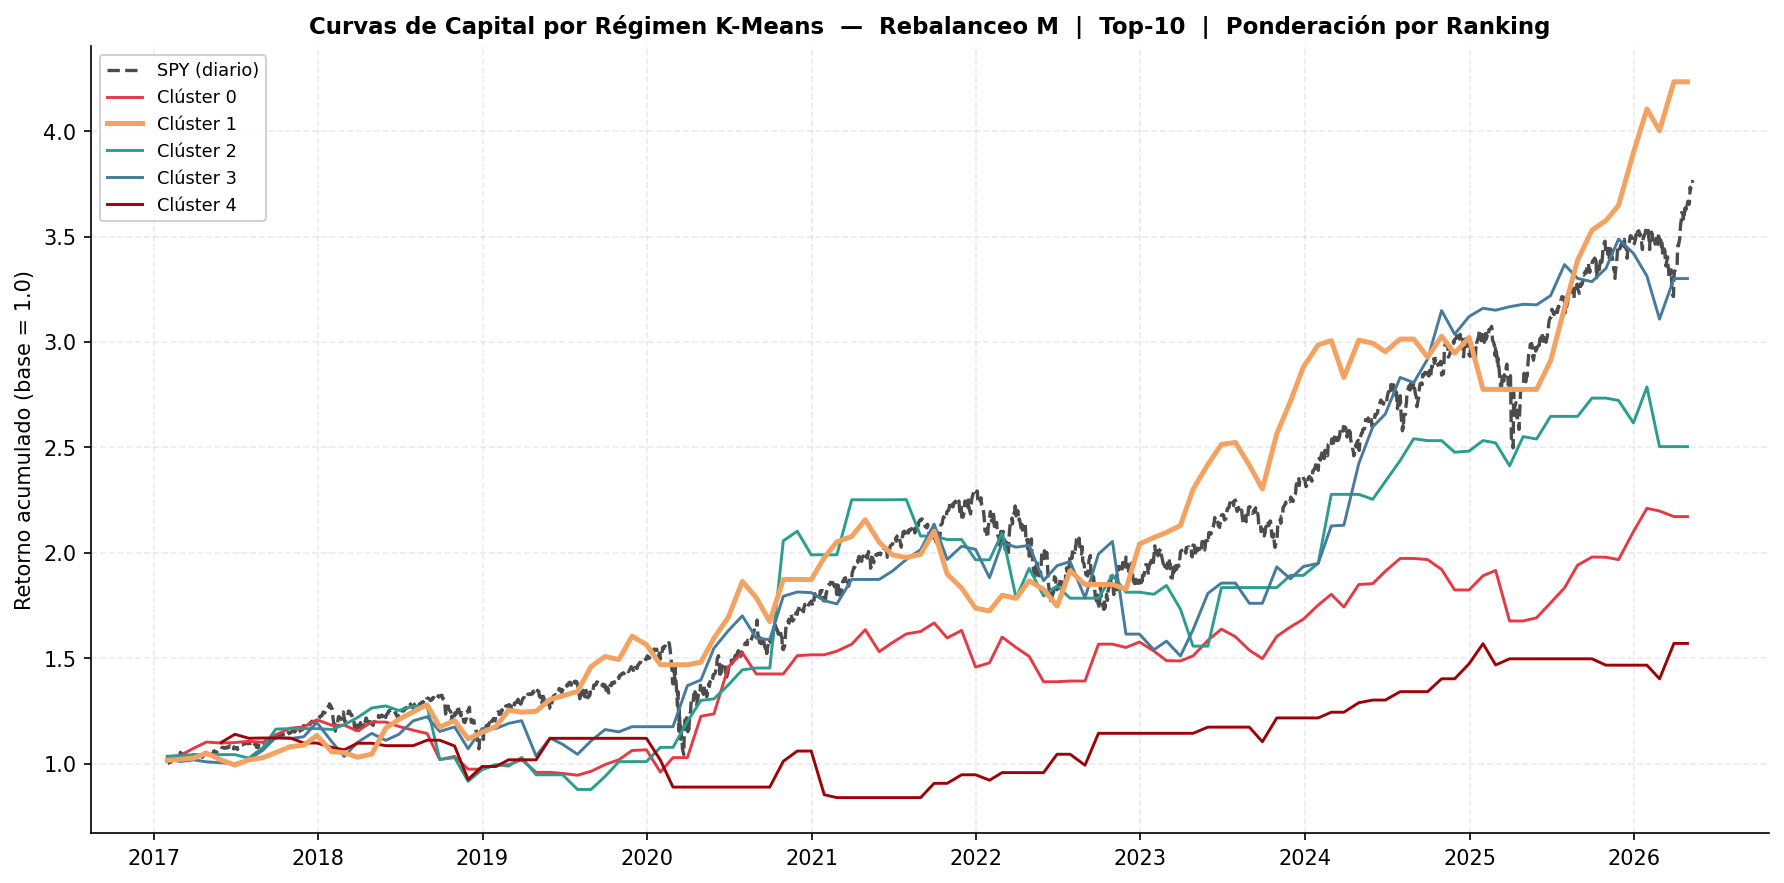
\includegraphics[width=0.95\textwidth]{media/equity_simple.png}
    \caption{Curvas de capital por régimen K-Means frente al benchmark SPY.}
    \label{fig:capital_clusters}
\end{figure}

De forma visual ya se aprecia que no todos los entornos de mercado ofrecen las mismas condiciones para una estrategia basada en \textit{momentum}. Algunos clústeres concentran fases especialmente favorables, mientras que otros presentan resultados más discretos o mayor inestabilidad.

\begin{table}[H]
\centering
\caption{Métricas principales por régimen de mercado. Rebalanceo mensual, Top-10 y ponderación por ranking.}
\label{tab:metricas_clusters}
\resizebox{\textwidth}{!}{%  <--- ESTA LÍNEA ES LA MAGIA
\begin{tabular}{lccccc}
\toprule
\textbf{Clúster} & \textbf{CAGR (\%)} & \textbf{Sharpe} & \textbf{MaxDD (\%)} & \textbf{Períodos Activos} & \textbf{SPY CAGR (\%)} \\
\midrule
0 --- Bajista moderado      & 8,66  & 0,531 & -21,80 & 97  & 11,79 \\
1 --- Bear market rally     & 16,72 & 1,002 & -20,06 & 101 & 11,79 \\
2 --- Alcista estable       & 10,33 & 0,462 & -31,13 & 74  & 11,79 \\
3 --- Pullback alcista      & 13,65 & 0,664 & -29,29 & 102 & 11,79 \\
4 --- Estrés/Capitulación   & 5,14  & 0,312 & -26,39 & 44  & 11,79 \\
\bottomrule
\end{tabular}
} % <--- NO TE OLVIDES DE CERRAR LA LLAVE AQUÍ
\end{table}

Los resultados, calculados mediante una diversificación \textit{Top-10}, muestran una diferenciación cuantitativa clara entre regímenes:

\begin{itemize}
    \item \textbf{Clúster 1 (Bear market rally):} Presenta el mejor comportamiento agregado de forma destacada, con un CAGR del 16,72\% y un ratio Sharpe de 1,002, batiendo ampliamente al \textit{benchmark}. El análisis de sus activos constituyentes más frecuentes (ej. Banco Santander, Ferrovial y activos defensivos como el oro a través de GLD) sugiere que, tras fases de sobreventa, las rotaciones agresivas hacia activos descorrelacionados o cíclicos ofrecen un \textit{alpha} significativo.
    
    \item \textbf{Clúster 3 (Pullback alcista):} Se consolida como un régimen altamente favorable, superando también al SPY con un CAGR del 13,65\% y un Sharpe robusto (0,664) respaldado por 102 períodos activos. Este dato confirma que comprar líderes de \textit{momentum} durante pequeñas correcciones dentro de tendencias estructurales positivas es una de las estrategias estadísticamente más fiables.
    
    \item \textbf{Clúster 2 (Alcista estable):} Muestra una rentabilidad positiva (10,33\%), pero ligeramente inferior al SPY. En mercados extremadamente complacientes y ordenados, el modelo \textit{Top-10} sufre porque la dispersión entre activos es menor; es decir, "todo sube", lo que diluye la ventaja comparativa del factor \textit{momentum}.
    
    \item \textbf{Clústeres 0 y 4 (Regímenes de debilidad y estrés):} Presentan los peores resultados relativos. Destaca especialmente el Clúster 4 (Capitulación), con apenas un 5,14\% de CAGR y un Sharpe deficiente de 0,312. Además, al observar los activos seleccionados durante este clúster (los propios índices SPY y QQQ), se infiere que el algoritmo colapsa y no encuentra acciones individuales que destaquen, refugiándose en el mercado general en medio del pánico.
\end{itemize}

En conjunto, los datos respaldan la idea central del trabajo: la rentabilidad ajustada al riesgo del factor \textit{momentum} no es constante, sino fuertemente asimétrica y dependiente del régimen de mercado detectado mediante K-Means.


% \parencite{Daniel2016}
% \parencite{Asness2013}

\subsection{Interpretación Económica de los Regímenes}

Más allá de la rentabilidad, los clústeres detectados presentan una lectura económica coherente:

\begin{itemize}
    \item \textbf{Bajista moderado:} fases de deterioro, sin capitulación extrema.
    
    \item \textbf{Bear market rally:} rebotes intensos tras caídas previas, normalmente acompañados de alta dispersión entre activos.
    
    \item \textbf{Alcista estable:} tendencia positiva sostenida, con volatilidad relativamente contenida.
    
    \item \textbf{Pullback alcista:} correcciones temporales dentro de un mercado estructuralmente favorable.
    
    \item \textbf{Estrés/Capitulación:} episodios de miedo generalizado, ventas forzadas o shocks externos.
\end{itemize}

Esta clasificación refuerza que el algoritmo no solo segmenta datos estadísticamente, sino que identifica contextos reconocibles desde el punto de vista financiero.

\subsection{Implicaciones para la Gestión de Cartera}

Una de las conclusiones más relevantes es que no todos los regímenes justifican el mismo nivel de exposición al riesgo. Si determinados clústeres concentran mejores métricas históricas, una aplicación práctica del modelo consistiría en modular el tamaño de la posición según el entorno detectado.

Por ejemplo:

\begin{itemize}
    \item Mayor exposición en clústeres 1 y 3.
    \item Exposición neutral o reducida en clúster 2.
    \item Perfil defensivo o incluso ausencia de señal en clústeres 0 y 4.
\end{itemize}

Este enfoque convertiría al sistema en una herramienta no solo de selección de activos, sino también de asignación.

%\subsection{Conclusión del Capítulo}

%Los resultados obtenidos muestran que la combinación de filtrado topológico (DBSCAN), segmentación por regímenes (K-Means) y selección por \textit{momentum} genera comportamientos diferenciados y económicamente interpretables.

%La evidencia empírica sugiere que adaptar la estrategia al contexto de mercado mejora la consistencia de los resultados frente a una aplicación indiscriminada del mismo modelo en cualquier entorno. En consecuencia, la detección previa del régimen se confirma como una capa de valor relevante dentro de la arquitectura propuesta.